\documentclass[aspectratio=169,11pt]{beamer}

% Shared style (ib-tutorials.sty at the repo root).
\makeatletter\def\input@path{{./}{../}}\makeatother
\usepackage{ib-tutorials}

\usepackage[utf8]{inputenc}
\usepackage{amsmath,amssymb}
\usepackage{booktabs}
\usepackage{array}
\newcolumntype{L}[1]{>{\raggedright\arraybackslash}p{#1}}
\usepackage{graphicx}
\usepackage{xcolor}
\usepackage{tikz}
\usetikzlibrary{arrows.meta,positioning,shapes.geometric,fit,calc}
\usepackage{hyperref}

\newcommand{\sourcecredit}[1]{\vfill\begin{flushright}\tiny\textcolor{DarkGray}{#1}\end{flushright}}
% One glossary table: term | meaning | chapters.
\newenvironment{glossarytable}{\scriptsize\renewcommand{\arraystretch}{1.08}%
  \begin{tabular}{@{}L{0.19\textwidth}L{0.63\textwidth}L{0.12\textwidth}@{}}\toprule
  term & meaning & chapters\\\midrule}{\bottomrule\end{tabular}}
% One reference: the chapters that cite it, in grey, after the entry.
\newcommand{\ch}[1]{\textcolor{DarkGray}{[#1]}}
\newcommand{\doi}[1]{\href{https://doi.org/#1}{doi:\detokenize{#1}}}
\newenvironment{reflist}{\scriptsize\begin{itemize}\setlength{\itemsep}{2.5pt}}{\end{itemize}}

\title[Appendix B: glossary, references, credits]{Appendix B: Glossary, references and credits}
\subtitle{The terms of the series with the chapters that teach them; every paper, book and program the chapters cite, in one list; who made what, the pictures from elsewhere, and the licences}
\author[Miller]{Laura A. Miller}
\institute[UArizona]{Department of Mathematics, University of Arizona}
\date{Using IB Software \textbullet\ Appendix B}

\begin{document}

% 1
\begin{frame}[plain]
\maketutorialtitlepanel{%
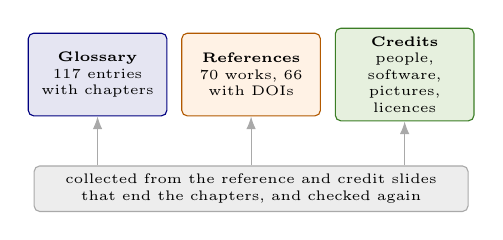
\begin{tikzpicture}[every node/.style={font=\tiny}, box/.style={draw, rounded corners=2pt, align=center, inner sep=3pt, text width=1.55cm, minimum height=1.05cm}]
  \node[box,draw=NavyBlue,fill=NavyBlue!10] (g) at (0,0) {\textbf{Glossary}\\117 entries\\with chapters};
  \node[box,draw=orange!70!black,fill=orange!10] (r) at (1.95,0) {\textbf{References}\\70 works, 66 with DOIs};
  \node[box,draw=OliveGreen,fill=OliveGreen!10] (c) at (3.9,0) {\textbf{Credits}\\people, software, pictures, licences};
  \node[draw=DarkGray,fill=LightGray!40,rounded corners=2pt,align=center,text width=5.3cm,inner sep=3pt] (s) at (1.95,-1.45) {collected from the reference and credit slides that end the chapters, and checked again};
  \draw[-{Latex[length=1.6mm]},DarkGray] (s.north -| g.south) -- (g.south);
  \draw[-{Latex[length=1.6mm]},DarkGray] (s.north -| r.south) -- (r.south);
  \draw[-{Latex[length=1.6mm]},DarkGray] (s.north -| c.south) -- (c.south);
\end{tikzpicture}}
\end{frame}

% 2
\begin{frame}{How to use this appendix}
\label{fr:use}
\begin{columns}[T,onlytextwidth]
\begin{column}{0.5\textwidth}
\small
\begin{itemize}\setlength{\itemsep}{3pt}
  \item \al{A word you do not know}: the glossary (slides \ref{fr:g1}--\ref{fr:g16}) gives its meaning in a line and the chapters that teach it, the main one first.
  \item \al{A paper a chapter cites}: the references (slides \ref{fr:r1}--\ref{fr:r10}) give it in full, with its DOI where it has one and every chapter that cites it; the talks, notes and tutorials are on slides \ref{fr:talks}--\ref{fr:talks2}.
  \item \al{The program behind a result}: the software slides (\ref{fr:sw1}--\ref{fr:sw3}) give the versions used.
  \item \al{Who made what, and what you may reuse}: the credits, pictures and licences (slides \ref{fr:people1}--\ref{fr:cite2}).
\end{itemize}
\end{column}
\begin{column}{0.47\textwidth}
\small Chapter labels: 0.1 and 0.2 are the front matter; 1--3 setting up (with 1b); 4a--4f IB2d; 5--16 IBAMR (with 8a, 8b, 9a, 9b); 17--25 IBFE; 26--33 VisIt; 34 and 35 Planktos; 36 the examples guide; X1--X4 the archive (legacy); A--C the appendices.
\vspace{2mm}
\begin{punchbox}
\small Each chapter's own References (and credits) slide stays the authority for that chapter, with the exact files, versions and course decks it drew on; this appendix gathers them and adds the cross-references.
\end{punchbox}
\end{column}
\end{columns}
\end{frame}

% ---------------------------------------------------------------- glossary
% 3
\begin{frame}{Glossary (1/16): A}
\label{fr:g1}
\begin{glossarytable}
active stress, active tension & An extra stress along the fibres of an IBFE body whose tension $T(\mathbf{s}, t) \ge 0$ the program prescribes in space and time (a contraction on a schedule, a travelling pulse, a pulse on one side: IBFE/06) to model muscle; IB2d's muscle models do the same with springs between points, and chapter 9b puts an active tension into a spring force. & 20; 4e, 9b\\
adaptive mesh refinement (AMR) & Finer Cartesian patches laid over a coarse grid where they are needed (around the structure, and optionally where the vorticity is large); IBAMR's grid is a hierarchy of such levels, managed by SAMRAI (IBAMR's fork of it). & 5, 7, 26, 33\\
advection--diffusion & Transport of a concentration by the flow and by diffusion: IBAMR's advection--diffusion integrators (IBFE/12) and IB2d's concentration option. & 24, 15, 7; 4a, 4b, 4e\\
agent, Swarm (Planktos) & An agent is one moving individual, an organism or a particle; a \code{Swarm} is a group of agents that move by one rule (the flow, noise, behaviour). & 34, 35\\
anchor (\code{.anchor}) & A file that gives the number of anchor points, then their indices, one per line; IBAMR keeps those points fixed where they start: they neither spread force to the fluid nor interpolate its velocity. & 6\\
autoibamr & The installer that downloads and builds IBAMR with the libraries it needs (PETSc, libMesh, SAMRAI, HDF5, Silo, Boost) in one command. & 2, 3\\
\end{glossarytable}
\end{frame}

% 4
\begin{frame}{Glossary (2/16): B--C}
\label{fr:g2}
\begin{glossarytable}
beam (\code{.beam}) & A bending force on three consecutive points: after the count, each line gives the three points, a bending rigidity and optionally a rest curvature, a vector of \code{NDIM} numbers (the preferred second difference $\mathbf{X}_i - 2\mathbf{X}_j + \mathbf{X}_k$); the middle point is the master. & 6, 10\\
boundary conditions (IBAMR) & Set side by side with muParser expressions \code{acoef}, \code{bcoef}, \code{gcoef}: $(a, b) = (1, 0)$ prescribes the velocity, $(0, 1)$ the traction; a direction can be periodic instead. & 7, 24\\
Brinkman term & A drag proportional to the velocity, set by a permeability field, that makes a region porous (IB2d's \code{brinkman}, MATLAB only; IBAMR's Brinkman penalization, chapter 14, is related); Planktos's \code{set\_brinkman\_flow} is the analytic flow in and over such a layer. & 4a, 4e; 35, 34; 14\\
CFL condition & The limit on an explicit time step, $|u|\,\Delta t/\Delta x \le C$ (Courant, Friedrichs and Lewy 1928); IBAMR's \code{cfl} key (\code{CFL\_MAX} at the top of the examples' inputs). One of several limits on \code{DT}. & 5, 16; 4d\\
CLI (VisIt) & VisIt's Python command line: \code{visit -cli} (with a window) or \code{visit -nowin -cli} (without); \code{visit -nowin -cli -s script.py -- \ldots} runs a script with its arguments, the way of this series. & 32, 31, 30, 27--29, 33; 4b\\
client--server (VisIt) & The window on your computer, the engine that reads the data on the cluster. & 31\\
\end{glossarytable}
\end{frame}

% 5
\begin{frame}{Glossary (3/16): C}
\label{fr:g3}
\begin{glossarytable}
CMake & The build system of IBAMR programs: each example's \code{CMakeLists.txt} finds IBAMR with \code{find\_package(IBAMR)} and builds \code{main2d} or \code{main3d}. & 3, 2, 15, 25\\
concentration & A scalar carried by the flow: IB2d's concentration solver and IBFE/12's advected field. & 4a, 4b, 4e; 24\\
ConstraintIB & IBAMR's method for rigid bodies and for bodies whose deformation is prescribed (a swimming eel): after each fluid solve the velocity inside the body is corrected to the body's, whose translation and rotation are either prescribed or computed from the momentum of the fluid in the body (free bodies, free swimmers) (Bhalla et al.\ 2013). & 14, 15\\
convergence, order of accuracy & How fast the error falls when the grid and the time step are refined: first order for thin elastic boundaries, higher for smooth problems (Griffith and Peskin 2005). & 4d, 5, 16\\
crosslink spring (\code{.xspring}) & A spring with global indices, so that it can join points of two structures on the same level; the line format of \code{.spring}. & 6, 9a\\
curvature (rest) & The preferred curvature of a beam, given as a vector: the preferred second difference of its three points, in units of length ($\kappa\,\Delta s^2$ for a curve of curvature $\kappa$); changing it in time bends a structure (IB/09, IB/10's jellyfish bell). & 10, 6\\
\end{glossarytable}
\end{frame}

% 6
\begin{frame}{Glossary (4/16): D--E}
\label{fr:g4}
\begin{glossarytable}
damping (target points) & The optional third number on a \code{.target} line: a dashpot, force $-\eta\,\mathbf{U}$, beside the tether spring. & 6, 8a, 9a\\
delta function (regularized) & The smooth kernel $\delta_h$ that spreads the structure's forces to the grid and interpolates the grid's velocity to the points; IBAMR's \code{delta\_fcn} (\code{IB\_4} in this series' inputs; \code{IB\_3}, \code{IB\_6}, B-splines). & 5, 4a, 17\\
dimensionless numbers & Ratios that decide which flows are alike: the Reynolds, Strouhal, Womersley and P\'eclet numbers, the force coefficients. & 8b, 8a\\
Displace operator (VisIt) & Moves a mesh by a vector variable, an IBFE mesh by its displacement \code{dX} for instance. & 28, 17, 27, 21, 22, 24\\
dumps.visit, visit\_dump & IBAMR's Eulerian output: SAMRAI's VisIt writer saves each dump as HDF5 files in a \code{visit\_dump.NNNNN} folder, and \code{dumps.visit} lists them for VisIt. & 26, 33, 3, 17, 28\\
Environment (Planktos) & The domain with its fluid velocity (read from IB2d's VTK output, IBAMR data exported to VTK, COMSOL VTU or NetCDF files, or generated analytically, such as the Brinkman layer) and its immersed meshes, in which a \code{Swarm} moves. & 34, 35\\
Euler--Maruyama & The stochastic version of Euler's method, for agents with Brownian noise (Milstein's scheme adds the next term, strong order 1 instead of 0.5, which matters when the noise depends on position). & 34, 35\\
\end{glossarytable}
\end{frame}

% 7
\begin{frame}{Glossary (5/16): E--F}
\label{fr:g5}
\begin{glossarytable}
Eulerian & Described on the fixed Cartesian grid, as the fluid is; the opposite of Lagrangian. & 5, 11\\
Exodus (ExodusII; \code{.ex2}, \code{.e}) & Sandia's netCDF-based (netCDF-4, so HDF5 underneath) mesh and field format, which libMesh reads and writes: IBFE's meshes from Cubit and its output (\code{output.ex2}), opened in VisIt. & 17, 18, 21, 23, 28, 33\\
explicit time stepping, stiffness & The structure's forces are computed from positions already known (the old ones, or IBAMR's midpoint predictions), not solved together with the new ones, so stiff springs, beams and target points need small time steps. & 5, 8a, 16; 4d, A\\
expression (VisIt) & A new variable defined from others: a magnitude, the vorticity, a value from another time or another mesh (\code{conn\_cmfe}, \code{pos\_cmfe}). & 28, 26, 27, 29\\
FE mesh & The finite-element mesh of an IBFE structure (triangles, quadrilaterals, tetrahedra, hexahedra), from gmsh, Triangle, TetGen, Cubit, MATLAB's PDE Toolbox or libMesh's own generators. & 17, 18\\
fibre direction & A unit vector $\mathbf{f}_0(\mathbf{s})$ of an IBFE body's reference configuration (a function of the reference position, or stored per element as a system on the mesh), along which a fibre stress, passive or active (chapter 20's is active), acts. & 20\\
force function (spring) & The fifth number on a \code{.spring} line: chooses how the force depends on the length; a program can register its own functions. & 9b, 6\\
\end{glossarytable}
\end{frame}

% 8
\begin{frame}{Glossary (6/16): F--H}
\label{fr:g6}
\begin{glossarytable}
FTLE & The finite-time Lyapunov exponent: how fast trajectories that start close together separate over a duration $\tau = T - t_0$ (Planktos's \code{T} is the end time); its ridges are candidate Lagrangian coherent structures (forward time: repelling; backward: attracting), to be read with care. Planktos computes it. & 34, 35, 33\\
generator & A MATLAB or Python script that writes an example's structure files (\code{generate\_mesh2d.m} / \code{.py}). & 6, A\\
gmsh & An open-source mesh generator: \code{.geo} scripts to \code{.msh} meshes (MSH 2.2 ASCII, the safe choice and what every example ships; libMesh also reads MSH 4.1 ASCII, but no binary MSH). & 18, 22, 1b\\
GriddingAlgorithm, CartesianGeometry & The SAMRAI input blocks that set the grid: the domain, the coarsest grid, the number of levels, the refinement ratio, the patch sizes. & 7, 3, 5, 12, 22, 23\\
HDF5 & A hierarchical data format: SAMRAI's VisIt dumps and IBAMR's restart files; \code{h5py} reads it in Python, \code{h5read} in MATLAB. & 33, 2\\
\end{glossarytable}
\end{frame}

% 9
\begin{frame}{Glossary (7/16): H--I}
\label{fr:g7}
\begin{glossarytable}
hier\_data\_IB2d & The folder (\code{data\_dump\_dirname}) that an example's own \code{output\_data} fills every \code{data\_dump\_interval} steps: in the IB examples (after IBAMR's \code{ex1}, without its HDF5 part) the Lagrangian positions \code{X.*} and forces \code{F.*} as PETSc ASCII vectors; in IBFE/01, 05, 06 and 12, only with \code{data\_dump\_interval} $> 0$, the velocity and pressure as SAMRAI HDF5 files (\code{hier\_data.NNNNN.samrai.PPPPP}) with the mesh and its equation systems; IBFE/10 writes its \code{tether\_force.txt} there. & 11, 3, 17, 22, 33\\
Hill model & A muscle model with a contractile element (Hill's force--velocity law) and elastic elements in series and in parallel; IB2d's three-element muscle (MATLAB; broken in Python), while its FV--LT muscle combines Hill's law with a length--tension curve. & 4e\\
IB method & The immersed boundary method: the fluid on a fixed grid, the structure as moving points that spread their forces to the fluid and move with its interpolated velocity (Peskin 2002). & 5\\
IB2d & Battista's immersed boundary code in 2D, in MATLAB (matIB2d) and Python (pyIB2d, ported by C. Strickland). & 4a--4f\\
IBAMR & Griffith's parallel, adaptive library for the immersed boundary method and its relatives (IBFE, ConstraintIB, IIM). & 2, 3, 5--25\\
IBFE & IBAMR's hybrid finite-difference/finite-element IB method: the structure is a finite-element mesh with a hyperelastic stress (Griffith and Luo 2017). & 17--25\\
\end{glossarytable}
\end{frame}

% 10
\begin{frame}{Glossary (8/16): I--J}
\label{fr:g8}
\begin{glossarytable}
IBTK & The IBAMR toolkit, the library under IBAMR (\code{IBTKInit}, \code{AppInitializer}, \code{LDataManager}, the solvers). & 23, 3, 9a, 17\\
IIM & The immersed interface method: the structure's forces enter as jump conditions across the interface; IBAMR's \code{examples/IIM}. & 15, 25\\
impedance pump & A valveless pump driven by squeezing an elastic tube away from its centre (Hickerson et al.\ 2005): IB2d's \code{Tracers\_In\_Impedance\_Pump} and dynamic-suction heart tubes, and IB/11's suction modes (chapter 9b's ``dynamic suction pumping'', Liebau's valveless pumping). & 4e, 4b, 9b\\
inertial particles & Particles with their own mass, which lag the flow (Maxey and Riley 1983; Haller and Sapsis 2008); Planktos's \code{inertial\_particles}. & 34, 35\\
input file (\code{input2d}, \code{input3d}) & The text file of constants and blocks that an IBAMR program reads at the start. & 3, 7\\
instrumentation (\code{.inst}) & Flow meters: points that define surfaces through which IBAMR integrates the flow rate and the pressure during the run. & 6, 15\\
interpolation, spreading & The two halves of the IB coupling: the grid's velocity is interpolated to the points, the points' forces are spread to the grid. & 5\\
job array (Slurm) & One \code{sbatch} submission that runs many tasks, each with its \code{SLURM\_ARRAY\_TASK\_ID}: a parameter sweep. & 3, 8a\\
\end{glossarytable}
\end{frame}

% 11
\begin{frame}{Glossary (9/16): K--L}
\label{fr:g9}
\begin{glossarytable}
KDE & A kernel density estimate: a smooth density of agent positions (Planktos plots the marginal ones along each axis), Gaussian, with Scott's bandwidth factor by default; Planktos's \code{dist="density"}. & 34, 35\\
kinematics (ConstraintIB) & The class that prescribes a body's velocity in time (\code{ConstraintIBKinematics}). & 14\\
Kirchhoff rod (\code{.rod}, \code{.director}) & Rods that resist bending and twisting, with a material frame at each point; no example of this series uses them. & 6, 15\\
Lagrangian & Described on material points that move with the structure; the opposite of Eulerian. & 5, 9a, 11\\
lag\_data.visit & IBAMR's Lagrangian output for VisIt (Silo files): the points and the meshes of their springs. & 28, 26\\
LCS & Lagrangian coherent structures: material lines that organize transport; FTLE ridges are candidates for them, to be read with care (Shadden et al.\ 2005; Haller 2015). & 33, 34, 35\\
level (AMR) & One refinement level of the patch hierarchy: level 0 is the coarsest, and each finer level divides the cells by the refinement ratio. & 5, 7\\
libMesh & The finite-element library under IBFE: meshes, Exodus input and output, quadrature. & 17, 18, 23\\
lineout (VisIt) & The values of a variable along a line, as a curve. & 29, 32, 33\\
\end{glossarytable}
\end{frame}

% 12
\begin{frame}{Glossary (10/16): M--N}
\label{fr:g10}
\begin{glossarytable}
mass (\code{.mass}) & Mass on a point by the penalty method: a massive copy of the point tied to it by a stiff spring (Kim and Peskin 2007); each line gives the index, the mass and the penalty stiffness. & 13, 6, 4e\\
Mesh plot (VisIt) & Draws the lines of a mesh: a structure's springs as lines, the AMR patches, an IBFE mesh. & 26, 28, 4b, 27\\
MeshmerizeMe & Senter's software that turns an SVG outline (from an image by its companion ContourizeMe, or drawn by hand) into IB2d and IBAMR \code{.vertex} points at $\Delta s = \Delta x/2$; the springs and targets are written by a script afterwards (Senter et al.\ 2021). & 4f, 1b\\
MPI & The message-passing library that runs a program as several processes: \code{mpirun -np 4}. & 2, 3, 31\\
muParser & The expression parser of IBAMR's input files: functions of the coordinates \code{X\_0}, \code{X\_1} and the time \code{t}. & 7, 23, 24\\
muscle model & See Hill model and active stress. & 4e, 20, 9b\\
Navier--Stokes equations & The equations of incompressible viscous flow that IBAMR solves on the grid. & 5\\
neo-Hookean & A hyperelastic material law, the usual first choice for an IBFE body; chapter 19 writes its PK1 stress. & 19\\
\end{glossarytable}
\end{frame}

% 13
\begin{frame}{Glossary (11/16): N--P}
\label{fr:g11}
\begin{glossarytable}
NORMALIZE\_\allowbreak{}PRESSURE & The examples' constant for the fluid integrator's key \code{normalize\_pressure} (default \code{FALSE}): \code{TRUE} removes the mean of the pressure every step, useful when every side is a velocity condition or periodic and the pressure is defined only up to a constant (the IB examples set it; the IBFE examples run with \code{FALSE}); with a traction (open) side the boundary fixes the level and it must stay \code{FALSE} (IB/13). & 7, 26\\
Open OnDemand & The web portal of the University of Arizona's cluster (Puma, its only one since August 2026): desktops, files, jobs. & 1, 31\\
operator (VisIt) & A transformation applied to a plot: Slice, Resample, Displace, Threshold, Box. & 26--28, 33\\
patch & A rectangular block of cells on one AMR level. & 5, 7, 26, 33\\
periodic & The box wraps around in a direction (\code{periodic\_dimension}), which overrides that direction's boundary blocks. & 7, 24, 12; 4a\\
PETSc & The linear-algebra library (vectors, Krylov solvers) that IBAMR uses; the \code{X.*} and \code{F.*} files of \code{hier\_data\_IB2d} are PETSc ASCII vectors. & 2, 11, 16\\
Pick (VisIt) & The value of a variable at a clicked point or zone. & 28, 29\\
PK1 stress & The first Piola--Kirchhoff stress, the function an IBFE program supplies: force per unit area of the reference configuration. & 19, 17\\
\end{glossarytable}
\end{frame}

% 14
\begin{frame}{Glossary (12/16): P--R}
\label{fr:g12}
\begin{glossarytable}
Planktos & A Python agent-based framework for small organisms in a flow (Strickland et al.\ 2022). & 34, 35\\
porous, poroelastic (IB2d) & Points that slip through the fluid at a rate set by a porosity coefficient (\code{.porous}), or that drift with their spring forces (\code{.poroelastic}). & 4a, 4e\\
Pseudocolor (VisIt) & A colour map of a scalar on the mesh. & 26, 4b, 27, 28\\
Puma & The University of Arizona's HPC cluster, for which the series' job scripts are written. & 1, 3, 31\\
pyIB2d, matIB2d & IB2d's Python and MATLAB versions. & 4a\\
quadrature points & The points inside each element where IBFE evaluates the stress and from which it spreads the force. & 17, 19, 18, 22\\
Query (VisIt) & A computed number (a minimum, a maximum, an integral, a flux), at one time or over time. & 29, 28\\
refinement ratio & The factor between the cell sizes of consecutive levels (2 or 4). & 7\\
regridding & Rebuilding the patches as the structure moves: when a point may have moved \code{REGRID\_CFL\_INTERVAL} cells (0.5 in the examples) or every \code{regrid\_interval} steps. & 5, 7\\
Resample (VisIt) & Interpolates a field onto a uniform grid; with Export Database it writes VTK files. & 33, 32, 31, 35\\
\end{glossarytable}
\end{frame}

% 15
\begin{frame}{Glossary (13/16): R--S}
\label{fr:g13}
\begin{glossarytable}
rest length & The length at which a spring exerts no force. & 6, 9a\\
restart files & The saved state from which a run can continue (\code{restart\_IB2d}). & 3, 23\\
Reynolds number & $\mathrm{Re} = \rho U L/\mu = UL/\nu$: inertial forces over viscous forces. & 8b\\
Robin boundary condition & $a\,u + b\,\partial u/\partial n = g$, the general form behind IBAMR's boundary blocks; for the velocity IBAMR accepts only $(a, b) = (1, 0)$, a velocity, and $(0, 1)$, where $g$ is a traction rather than a derivative; true Robin conditions are for scalars (chapter 24). & 7, 24\\
SAMRAI & LLNL's structured adaptive mesh refinement framework under IBAMR, in IBAMR's fork (IBSAMRAI2): the patch hierarchy, the input database, the VisIt writer. & 2, 7, 23, 33, 5\\
session file (VisIt) & The saved plots and settings of a VisIt window. & 26, 30, 4b, 28\\
Silo & An LLNL file format that VisIt reads; IBAMR writes its Lagrangian data in it. & 28, 33, 2\\
Slice (VisIt) & A plane cut through 3D data. & 27, 22, 33\\
Slurm & The job scheduler of the cluster: \code{sbatch}, \code{squeue}, job arrays. & 1, 3, 31\\
source (\code{.source}) & Fluid sources and sinks attached to points, each with a radius; the program sets their strengths in time. & 6, 15\\
\end{glossarytable}
\end{frame}

% 16
\begin{frame}{Glossary (14/16): S}
\label{fr:g14}
\begin{glossarytable}
sponge layer & An Eulerian body force (\code{SpongeLayerForceFunction}) that, within a distance \code{width} of a chosen face, damps chosen velocity components toward zero, e.g.\ to keep recirculation from re-entering at an outflow; in IBAMR's \code{ex7} its keys are misspelt and it is off. & 23\\
spring (\code{.spring}) & A spring between two points, linear by default: after the count, each line gives the two indices, the stiffness $\kappa$, the rest length $L$ (required) and optionally a force-function index with that function's extra parameters. & 6, 9a, 9b\\
stiffness & The $\kappa$ numbers in the structure files; they scale with the point spacing $\Delta s$. & 6, 8a\\
Stokes solver & The linear solver for the velocity and the pressure in each time step. & 16, 3, 5, 15\\
Strouhal number & $\mathrm{St}_L = fL/U$ with a length $L$ (the convention of this series and the theory series: the dimensionless frequency; about 0.2 for a cylinder's shedding with $L = D$), or $\mathrm{St}_A = fA/U$ with the stroke amplitude $A$ (the convention for flapping and swimming animals, Taylor et al.\ 2003): the frequency of a motion against the flow. & 8b\\
structure files & \code{.vertex}, \code{.spring}, \code{.beam}, \code{.target}, \code{.anchor}, \code{.mass}, \code{.xspring}, \code{.rod}, \code{.director}, \code{.inst}, \code{.source}. & 6\\
\end{glossarytable}
\end{frame}

% 17
\begin{frame}{Glossary (15/16): T--V}
\label{fr:g15}
\begin{glossarytable}
target point (\code{.target}) & A point tied by a stiff zero-length spring (and optional damping) to a target position, which the program may move. & 6, 9a\\
tether (IBFE) & A penalty body force $\kappa_s(\mathbf{s}_{\mathrm{target}} - \mathbf{X})$ (optionally with a damping term on the velocity, chapter 19) that holds an IBFE body near a target configuration, fixed ($\mathbf{s}_{\mathrm{target}} = \mathbf{s}$) or moved by the program (IBFE/01): the IBFE counterpart of target points. & 17, 19, 21, 22\\
time step (\code{DT}) & $\Delta t$, limited by the CFL condition and by the structure's stiffness. & 5, 16, 7, 8a; 4d\\
tracers (IB2d) & Massless points carried by the flow, written for VisIt. & 4b, 4a, 4e\\
traction condition & Prescribes the stress on a side, $(a, b) = (0, 1)$. & 7\\
Triangle & Shewchuk's 2D quality mesh generator (\code{.poly} input). & 18, 17\\
upstream examples & The examples shipped with IBAMR itself (\code{examples/IB}, \code{IBFE}, \code{ConstraintIB}, \code{IIM}, \ldots). & 15, 25\\
vertex (\code{.vertex}) & The count $N$, then $N$ lines of the Lagrangian points' coordinates. & 6\\
Vicsek model & Agents align with their neighbours' headings, with noise. & 35, 34\\
VisIt & LLNL's visualization and analysis tool, used throughout. & 26--33\\
\end{glossarytable}
\end{frame}

% 18
\begin{frame}{Glossary (16/16): V--W}
\label{fr:g16}
\begin{glossarytable}
viz\_IB2d, viz\_IB3d & The folders of IBAMR's visualization output (\code{dumps.visit}, \code{lag\_data.visit}, and IBFE's \code{output.ex2}); IB2d writes its VTK files to a \code{viz\_IB2d} folder too. & 3, 26, 17; 4b\\
vorticity & $\omega = \nabla\times\mathbf{u}$, the local rotation of the fluid (\code{Omega} in IBAMR's output). & 26, 27\\
VTK (legacy \code{.vtk}) & Kitware's text or binary format: IB2d's output and VisIt's resampled exports. & 4b, 33, 4a, 28, 35\\
Womersley number & $\alpha = R\sqrt{\omega/\nu}$, with $R$ the radius or half-width and $\omega = 2\pi f$: oscillation against viscosity in a pulsatile flow. & 8b\\
WSL; X11 forwarding & The Windows Subsystem for Linux, on which this series built and ran IBAMR on a desktop PC; \code{ssh -X}, a cluster program's windows on your screen. & 2, 36; 31\\
\end{glossarytable}
\end{frame}

% ---------------------------------------------------------------- references
% r1
\begin{frame}{References (1/10): Alberts -- Bhalla}
\label{fr:r1}
\begin{reflist}
  \item B. Alberts, A. Johnson, J. Lewis, M. Raff, K. Roberts and P. Walter. \emph{Molecular Biology of the Cell}, 4th ed. Garland Science, 2002. Figures 16-69 and 16-71, redrawn after the 2015 muscle lecture. \ch{4e}
  \item Y. Bao, J. Kaye and C. S. Peskin. A Gaussian-like immersed-boundary kernel with three continuous derivatives and improved translational invariance. \emph{J.\ Comput.\ Phys.} 316:139--144, 2016. \doi{10.1016/j.jcp.2016.04.024} \ch{5}
  \item A. W. Barrett. \emph{An adaptive viscoelastic fluid solver: formulation, verification, and applications to fluid--structure interaction}. PhD dissertation, University of North Carolina at Chapel Hill, 2019. \ch{15, 25}
  \item N. A. Battista, A. J. Baird and L. A. Miller. A mathematical model and MATLAB code for muscle--fluid--structure simulations. \emph{Integr.\ Comp.\ Biol.} 55(5):901--911, 2015. \doi{10.1093/icb/icv102} \ch{4a, 4b, 4e, 36}
  \item N. A. Battista, W. C. Strickland and L. A. Miller. IB2d: a Python and MATLAB implementation of the immersed boundary method. \emph{Bioinspir.\ Biomim.} 12(3):036003, 2017. \doi{10.1088/1748-3190/aa5e08}; arXiv:1610.07944. \ch{4a, 4b, 4d, 4e, 5, 6, 34, 35, 36}
  \item N. A. Battista, W. C. Strickland, A. Barrett and L. A. Miller. IB2d Reloaded: a more powerful Python and MATLAB implementation of the immersed boundary method. \emph{Math.\ Meth.\ Appl.\ Sci.} 41(18):8455--8480, 2018. \doi{10.1002/mma.4708}; arXiv:1707.06928. \ch{4a, 4b, 4d, 4e, 36}
  \item A. P. S. Bhalla, R. Bale, B. E. Griffith and N. A. Patankar. A unified mathematical framework and an adaptive numerical method for fluid--structure interaction with rigid, deforming, and elastic bodies. \emph{J.\ Comput.\ Phys.} 250:446--476, 2013. \doi{10.1016/j.jcp.2013.04.033} \ch{14, 15, 25, 36}
\end{reflist}
\sourcecredit{Every entry is the one on the cited chapters' References slides, completed (full author lists, issue numbers, DOIs) where they were short.}
\end{frame}

% r2
\begin{frame}{References (2/10): Bomphrey -- Ellington}
\label{fr:r2}
\begin{reflist}
  \item R. J. Bomphrey, T. Nakata, N. Phillips and S. M. Walker. Smart wing rotation and trailing-edge vortices enable high frequency mosquito flight. \emph{Nature} 544(7648):92--95, 2017. \doi{10.1038/nature21727} \ch{1b}
  \item J. Bonet and R. D. Wood. \emph{Nonlinear Continuum Mechanics for Finite Element Analysis}, 2nd ed. Cambridge University Press, 2008. \doi{10.1017/CBO9780511755446} \ch{19}
  \item H. C. Brinkman. A calculation of the viscous force exerted by a flowing fluid on a dense swarm of particles. \emph{Appl.\ Sci.\ Res.} A1(1):27--34, 1949. \doi{10.1007/BF02120313} \ch{35}
  \item H. Childs, E. Brugger, B. Whitlock, J. Meredith, S. Ahern, D. Pugmire, K. Biagas, M. C. Miller, C. Harrison, G. H. Weber, H. Krishnan, T. Fogal, A. Sanderson, C. Garth, E. W. Bethel, D. Camp, O. R\"ubel, M. Durant, J. M. Favre and P. Navr\'atil. VisIt: an end-user tool for visualizing and analyzing very large data. In E. W. Bethel, H. Childs and C. Hansen (eds.), \emph{High Performance Visualization: Enabling Extreme-Scale Scientific Insight}, Chapman and Hall/CRC, 2012, 357--372. \doi{10.1201/b12985} \ch{26, 27, 29, 30, 31, 32}
  \item R. Courant, K. Friedrichs and H. Lewy. \"Uber die partiellen Differenzengleichungen der mathematischen Physik. \emph{Math.\ Ann.} 100(1):32--74, 1928. \doi{10.1007/BF01448839} \ch{5}
  \item J. R. Dormand and P. J. Prince. A family of embedded Runge--Kutta formulae. \emph{J.\ Comput.\ Appl.\ Math.} 6(1):19--26, 1980. \doi{10.1016/0771-050X(80)90013-3} \ch{34, 35}
  \item C. P. Ellington. The aerodynamics of hovering insect flight. II. Morphological parameters. \emph{Phil.\ Trans.\ R. Soc.\ Lond.\ B} 305(1122):17--40, 1984. \doi{10.1098/rstb.1984.0050} \ch{12}
\end{reflist}
\end{frame}

% r3
\begin{frame}{References (3/10): Geuzaine -- Griffith}
\label{fr:r3}
\begin{reflist}
  \item C. Geuzaine and J.-F. Remacle. Gmsh: a 3-D finite element mesh generator with built-in pre- and post-processing facilities. \emph{Int.\ J.\ Numer.\ Meth.\ Engng} 79(11):1309--1331, 2009 (gmsh.info cites it as ``a three-dimensional finite element mesh generator''). \doi{10.1002/nme.2579} \ch{1b, 18, 22}
  \item A. M. Gordon, A. F. Huxley and F. J. Julian. The variation in isometric tension with sarcomere length in vertebrate muscle fibres. \emph{J.\ Physiol.} 184(1):170--192, 1966. \doi{10.1113/jphysiol.1966.sp007909} \ch{4e}
  \item B. E. Griffith. On the volume conservation of the immersed boundary method. \emph{Commun.\ Comput.\ Phys.} 12(2):401--432, 2012. \doi{10.4208/cicp.120111.300911s} \ch{4d}
  \item B. E. Griffith, R. D. Hornung, D. M. McQueen and C. S. Peskin. An adaptive, formally second order accurate version of the immersed boundary method. \emph{J.\ Comput.\ Phys.} 223(1):10--49, 2007. \doi{10.1016/j.jcp.2006.08.019} \ch{5}
  \item B. E. Griffith and S. Lim. Simulating an elastic ring with bend and twist by an adaptive generalized immersed boundary method. \emph{Commun.\ Comput.\ Phys.} 12(2):433--461, 2012. \doi{10.4208/cicp.190211.060811s} \ch{15}
  \item B. E. Griffith and X. Luo. Hybrid finite difference/finite element immersed boundary method. \emph{Int.\ J.\ Numer.\ Meth.\ Biomed.\ Engng} 33(12):e2888, 2017. \doi{10.1002/cnm.2888}; arXiv:1612.05916. \ch{5, 15, 17, 19, 20, 25, 28}
  \item B. E. Griffith and N. A. Patankar. Immersed methods for fluid--structure interaction. \emph{Annu.\ Rev.\ Fluid Mech.} 52:421--448, 2020 (free full text: PMC7531444). \doi{10.1146/annurev-fluid-010719-060228} \ch{5}
\end{reflist}
\end{frame}

% r4
\begin{frame}{References (4/10): Griffith -- Holzapfel}
\label{fr:r4}
\begin{reflist}
  \item B. E. Griffith and C. S. Peskin. On the order of accuracy of the immersed boundary method: higher order convergence rates for sufficiently smooth problems. \emph{J.\ Comput.\ Phys.} 208(1):75--105, 2005. \doi{10.1016/j.jcp.2005.02.011} \ch{4d, 5, 16}
  \item G. Haller. Lagrangian coherent structures. \emph{Annu.\ Rev.\ Fluid Mech.} 47:137--162, 2015. \doi{10.1146/annurev-fluid-010313-141322} \ch{34, 35}
  \item G. Haller and T. Sapsis. Where do inertial particles go in fluid flows? \emph{Physica D} 237(5):573--583, 2008. \doi{10.1016/j.physd.2007.09.027} \ch{34, 35}
  \item C. L. Hamlet, W. C. Strickland, N. Battista and L. A. Miller. Multiscale flow between the branches and polyps of gorgonians. \emph{J.\ Exp.\ Biol.} 226(5):jeb244520, 2023 (CC BY 4.0; in \code{papers/}). \doi{10.1242/jeb.244520} \ch{34, 35}
  \item G. Herschlag and L. A. Miller. Reynolds number limits for jet propulsion: a numerical study of simplified jellyfish. \emph{J.\ Theor.\ Biol.} 285(1):84--95, 2011. \doi{10.1016/j.jtbi.2011.05.035} \ch{10}
  \item A. I. Hickerson, D. Rinderknecht and M. Gharib. Experimental study of the behavior of a valveless impedance pump. \emph{Exp.\ Fluids} 38(4):534--540, 2005. \doi{10.1007/s00348-005-0946-z} \ch{4e}
  \item A. V. Hill. The heat of shortening and the dynamic constants of muscle. \emph{Proc.\ R. Soc.\ Lond.\ B} 126(843):136--195, 1938. \doi{10.1098/rspb.1938.0050} \ch{4e}
  \item G. A. Holzapfel. \emph{Nonlinear Solid Mechanics: A Continuum Approach for Engineering}. Wiley, 2000. \ch{19}
\end{reflist}
\end{frame}

% r5
\begin{frame}{References (5/10): Hoover -- Kolahdouz}
\label{fr:r5}
\begin{reflist}
  \item A. P. Hoover, B. E. Griffith and L. A. Miller. Quantifying performance in the medusan mechanospace with an actively swimming three-dimensional jellyfish model. \emph{J.\ Fluid Mech.} 813:1112--1155, 2017. \doi{10.1017/jfm.2017.3} \ch{20}
  \item A. P. Hoover, N. W. Xu, B. J. Gemmell, S. P. Colin, J. H. Costello, J. O. Dabiri and L. A. Miller. Neuromechanical wave resonance in jellyfish swimming. \emph{Proc.\ Natl.\ Acad.\ Sci.\ USA} 118(11):e2020025118, 2021. \doi{10.1073/pnas.2020025118} \ch{1b}
  \item A. F. Huxley. Muscle structure and theories of contraction. \emph{Prog.\ Biophys.\ Biophys.\ Chem.} 7:255--318, 1957. \doi{10.1016/S0096-4174(18)30128-8} \ch{4e}
  \item B. Kallemov, A. P. S. Bhalla, B. E. Griffith and A. Donev. An immersed boundary method for rigid bodies. \emph{Commun.\ Appl.\ Math.\ Comput.\ Sci.} 11(1):79--141, 2016. \doi{10.2140/camcos.2016.11.79} \ch{15}
  \item J. Keener and J. Sneyd. \emph{Mathematical Physiology II: Systems Physiology}, 2nd ed. Springer, 2009; chapter 15 (muscle), for further reading. \doi{10.1007/978-0-387-79388-7} \ch{4e}
  \item Y. Kim and C. S. Peskin. Penalty immersed boundary method for an elastic boundary with mass. \emph{Phys.\ Fluids} 19(5):053103, 2007. \doi{10.1063/1.2734674} \ch{13, 15}
  \item P. E. Kloeden and E. Platen. \emph{Numerical Solution of Stochastic Differential Equations}. Springer, 1992. \doi{10.1007/978-3-662-12616-5} \ch{34, 35}
  \item E. M. Kolahdouz, A. P. S. Bhalla, B. A. Craven and B. E. Griffith. An immersed interface method for discrete surfaces. \emph{J.\ Comput.\ Phys.} 400:108854, 2020. \doi{10.1016/j.jcp.2019.07.052} \ch{15}
\end{reflist}
\end{frame}

% r6
\begin{frame}{References (6/10): Kolahdouz -- Maxey}
\label{fr:r6}
\begin{reflist}
  \item E. M. Kolahdouz, A. P. S. Bhalla, L. N. Scotten, B. A. Craven and B. E. Griffith. A sharp interface Lagrangian--Eulerian method for rigid-body fluid--structure interaction. \emph{J.\ Comput.\ Phys.} 443:110442, 2021. \doi{10.1016/j.jcp.2021.110442} \ch{15}
  \item S. Kupfner Johnson and P. Hallock. A review of symbiotic gorgonian research in the western Atlantic and Caribbean with recommendations for future work. \emph{Coral Reefs} 39(2):239--258, 2020. \doi{10.1007/s00338-020-01891-0} \ch{34, 35}
  \item R. J. LeVeque. \emph{Finite Difference Methods for Ordinary and Partial Differential Equations: Steady-State and Time-Dependent Problems}. SIAM, 2007; chapters 7 (absolute stability) and 9 (the heat equation). \doi{10.1137/1.9780898717839} \ch{4d}
  \item S. Lim. Dynamics of an open elastic rod with intrinsic curvature and twist in a viscous fluid. \emph{Phys.\ Fluids} 22(2):024104, 2010. \doi{10.1063/1.3326075} \ch{15}
  \item X. Y. Luo and T. J. Pedley. A numerical simulation of unsteady flow in a two-dimensional collapsible channel. \emph{J.\ Fluid Mech.} 314:191--225, 1996. \doi{10.1017/S0022112096000286} \ch{23}
  \item R. W. Lymn and E. W. Taylor. Mechanism of adenosine triphosphate hydrolysis by actomyosin. \emph{Biochemistry} 10(25):4617--4624, 1971. \doi{10.1021/bi00801a004} \ch{4e}
  \item M. R. Maxey and J. J. Riley. Equation of motion for a small rigid sphere in a nonuniform flow. \emph{Phys.\ Fluids} 26(4):883--889, 1983. \doi{10.1063/1.864230} \ch{34, 35}
\end{reflist}
\end{frame}

% r7
\begin{frame}{References (7/10): McMillen -- Peskin}
\label{fr:r7}
\begin{reflist}
  \item T. McMillen, T. Williams and P. Holmes. Nonlinear muscles, passive viscoelasticity and body taper conspire to create neuromechanical phase lags in anguilliform swimmers. \emph{PLoS Comput.\ Biol.} 4(8):e1000157, 2008. \doi{10.1371/journal.pcbi.1000157} \ch{4e}
  \item O. Mesnard and L. A. Barba. Reproducible and replicable computational fluid dynamics: it's harder than you think. \emph{Comput.\ Sci.\ Eng.} 19(4):44--55, 2017. \doi{10.1109/MCSE.2017.3151254}; arXiv:1605.04339. \ch{1b}
  \item L. A. Miller. \emph{Fluid Dynamics and IBM Theory}, the companion series (2026). \url{https://github.com/fairyflies9/Fluid-Dynamics-and-IBM-Theory} \ch{0.1, 0.2, 4a, 5, 8b, 17, 19, 20}
  \item L. A. Miller and C. S. Peskin. When vortices stick: an aerodynamic transition in tiny insect flight. \emph{J.\ Exp.\ Biol.} 207(17):3073--3088, 2004. \doi{10.1242/jeb.01138} \ch{21}
  \item N. Nangia, H. Johansen, N. A. Patankar and A. P. S. Bhalla. A moving control volume approach to computing hydrodynamic forces and torques on immersed bodies. \emph{J.\ Comput.\ Phys.} 347:437--462, 2017. \doi{10.1016/j.jcp.2017.06.047} \ch{14}
  \item M. K. Ozalp, L. A. Miller, T. Dombrowski, M. Braye, T. Dix, L. Pongracz, R. Howell, D. Klotsa, V. Pasour and W. C. Strickland. Experiments and agent based models of zooplankton movement within complex flow environments. \emph{Biomimetics} 5(1):2, 2020. \doi{10.3390/biomimetics5010002} \ch{34}
  \item C. S. Peskin. The immersed boundary method. \emph{Acta Numerica} 11:479--517, 2002. \doi{10.1017/S0962492902000077} \ch{4a, 4d, 5, 6, 8b, 10, 16}
  \item C. S. Peskin and B. F. Printz. Improved volume conservation in the computation of flows with immersed elastic boundaries. \emph{J.\ Comput.\ Phys.} 105(1):33--46, 1993. \doi{10.1006/jcph.1993.1051} \ch{4d}
\end{reflist}
\end{frame}

% r8
\begin{frame}{References (8/10): Roma -- Shewchuk}
\label{fr:r8}
\begin{reflist}
  \item A. M. Roma, C. S. Peskin and M. J. Berger. An adaptive version of the immersed boundary method. \emph{J.\ Comput.\ Phys.} 153(2):509--534, 1999. \doi{10.1006/jcph.1999.6293} \ch{5}
  \item T. Sakurai, K. Yoshimatsu, N. Okamoto and K. Schneider. Volume penalization for inhomogeneous Neumann boundary conditions modeling scalar flux in complicated geometry. \emph{J.\ Comput.\ Phys.} 390:452--469, 2019. \doi{10.1016/j.jcp.2019.04.008} \ch{15}
  \item M. Santiago, N. A. Battista, L. A. Miller and S. Khatri. Passive concentration dynamics incorporated into the library IB2d, a two-dimensional implementation of the immersed boundary method. \emph{Bioinspir.\ Biomim.} 17(3):036003, 2022. \doi{10.1088/1748-3190/ac4afa} \ch{4a, 4b}
  \item D. W. Scott. \emph{Multivariate Density Estimation: Theory, Practice, and Visualization}. Wiley, 1992. \doi{10.1002/9780470316849} \ch{34, 35}
  \item D. M. Senter, D. R. Douglas, W. C. Strickland, S. G. Thomas, A. M. Talkington, L. A. Miller and N. A. Battista. A semi-automated finite difference mesh creation method for use with immersed boundary software IB2d and IBAMR. \emph{Bioinspir.\ Biomim.} 16(1):016008, 2021. \doi{10.1088/1748-3190/ababb0} \ch{1b, 4a, 4f, 6, 36}
  \item S. C. Shadden, F. Lekien and J. E. Marsden. Definition and properties of Lagrangian coherent structures from finite-time Lyapunov exponents in two-dimensional aperiodic flows. \emph{Physica D} 212(3--4):271--304, 2005. \doi{10.1016/j.physd.2005.10.007} \ch{34, 35}
  \item J. R. Shewchuk. Triangle: engineering a 2D quality mesh generator and Delaunay triangulator. In M. C. Lin and D. Manocha (eds.), \emph{Applied Computational Geometry: Towards Geometric Engineering}, LNCS 1148, Springer, 1996, 203--222. \doi{10.1007/BFb0014497} \ch{18}
\end{reflist}
\end{frame}

% r9
\begin{frame}{References (9/10): Si -- Turek}
\label{fr:r9}
\begin{reflist}
  \item H. Si. TetGen, a Delaunay-based quality tetrahedral mesh generator. \emph{ACM Trans.\ Math.\ Softw.} 41(2):11, 2015. \doi{10.1145/2629697} \ch{18}
  \item W. C. Strickland, N. A. Battista, C. L. Hamlet and L. A. Miller. Planktos: an agent-based modeling framework for small organism movement and dispersal in a fluid environment with immersed structures. \emph{Bull.\ Math.\ Biol.} 84(7):72, 2022. \doi{10.1007/s11538-022-01027-1} \ch{34, 35, 36}
  \item W. C. Strickland, L. A. Miller, A. Santhanakrishnan, C. Hamlet, N. A. Battista and V. Pasour. Three-dimensional low Reynolds number flows near biological filtering and protective layers. \emph{Fluids} 2(4):62, 2017. \doi{10.3390/fluids2040062} \ch{35}
  \item G. K. Taylor, R. L. Nudds and A. L. R. Thomas. Flying and swimming animals cruise at a Strouhal number tuned for high power efficiency. \emph{Nature} 425(6959):707--711, 2003. \doi{10.1038/nature02000} \ch{8b}
  \item R. Thirumalaisamy, N. A. Patankar and A. P. S. Bhalla. Handling Neumann and Robin boundary conditions in a fictitious domain volume penalization framework. \emph{J.\ Comput.\ Phys.} 448:110726, 2022. \doi{10.1016/j.jcp.2021.110726} \ch{15}
  \item S. Turek and J. Hron. Proposal for numerical benchmarking of fluid--structure interaction between an elastic object and laminar incompressible flow. In H.-J. Bungartz and M. Sch\"afer (eds.), \emph{Fluid--Structure Interaction: Modelling, Simulation, Optimisation}, Lecture Notes in Computational Science and Engineering 53, Springer, 2006, 371--385. \doi{10.1007/3-540-34596-5_15} \ch{4e, 15, 25, 28}
\end{reflist}
\end{frame}

% r10
\begin{frame}{References (10/10): Tytell -- Zhu}
\label{fr:r10}
\begin{reflist}
  \item E. D. Tytell, C.-Y. Hsu, T. L. Williams, A. H. Cohen and L. J. Fauci. Interactions between internal forces, body stiffness, and fluid environment in a neuromechanical model of lamprey swimming. \emph{Proc.\ Natl.\ Acad.\ Sci.\ USA} 107(46):19832--19837, 2010. \doi{10.1073/pnas.1011564107} \ch{4e}
  \item T. Vicsek, A. Czir\'ok, E. Ben-Jacob, I. Cohen and O. Shochet. Novel type of phase transition in a system of self-driven particles. \emph{Phys.\ Rev.\ Lett.} 75(6):1226--1229, 1995. \doi{10.1103/PhysRevLett.75.1226} \ch{34, 35}
  \item S. Vogel. \emph{Life in Moving Fluids: The Physical Biology of Flow}, 2nd ed. (revised and expanded). Princeton University Press, 1994. \doi{10.1515/9780691212975} \ch{8b}
  \item T. L. Williams, G. Bowtell and N. A. Curtin. Predicting force generation by lamprey muscle during applied sinusoidal movement using a simple dynamic model. \emph{J.\ Exp.\ Biol.} 201(6):869--875, 1998. \doi{10.1242/jeb.201.6.869} \ch{4e}
  \item L. Zhu and C. S. Peskin. Simulation of a flapping flexible filament in a flowing soap film by the immersed boundary method. \emph{J.\ Comput.\ Phys.} 179(2):452--468, 2002. \doi{10.1006/jcph.2002.7066} \ch{15}
\end{reflist}
\end{frame}

% 26
\begin{frame}{Talks, notes and tutorials cited (1/2)}
\label{fr:talks}
\scriptsize
\begin{itemize}\setlength{\itemsep}{2pt}
  \item N. A. Battista and L. A. Miller, ``Fluid Structure Interaction (FSI) and the Immersed Boundary Method (IB)'' (talk, 7 September 2016). \ch{4e}
  \item L. A. Miller, ``Quick introduction to muscle models'' (15 September 2015) and ``Muscle Activation Tutorial: the biology and Ca$^{2+}$ models''. \ch{4e}
  \item L. A. Miller, \emph{Software for Computational Fluid Dynamics, Part 1}, AIMEC--NSF Joint Workshop for the Model Species Cassiopea (2024). \ch{1b}
  \item M. Senter, ``Creating a Curvilinear Mesh from B\'ezier Curves'', design notes for an early C++ version of MeshmerizeMe (UNC Chapel Hill, about 2017). \ch{4f}
  \item K. Giesbrecht, L. A. Miller and J. Shi, ``A theoretical study of two-point dynamic suction pumping'' (poster, 2019--2020). \ch{9b}
  \item L. Waldrop, ``Data analysis in VisIt'', MATH 769 (16 February 2015; its 2017 version for IB2d's output). \ch{29, 30}
  \item G. Hobson, ``Post-Processing IBAMR Simulation Data in VisIt on a Computing Cluster: A Tutorial'' (Scripps Institution of Oceanography, UC San Diego, 23 September 2020), and its University of Arizona version. \ch{31, 32}
\end{itemize}
\end{frame}

% talks 2
\begin{frame}{Talks, notes and tutorials cited (2/2)}
\label{fr:talks2}
\scriptsize
\begin{itemize}\setlength{\itemsep}{2pt}
  \item N. Battista, ``Running IBAMR/IBFE on super computers'' (2014; UA version 2024) \ch{1, 3}; ``Part III: Let's make groovy movies!'' in the Kure/Killdevil tutorial (2014) \ch{30}; ``How To Make Simple Geometries in Gmsh'' (24 September 2014) \ch{18}.
  \item ``Getting started with Planktos'' (Miller lab, 2021). \ch{34, 35}
  \item P. Kelly, \emph{Solid Mechanics Lecture Notes, Part III: Foundations of Continuum Mechanics} (University of Auckland), section 3.5 on the stress measures \ch{19}; B. Griffith's 2009 MBI workshop slides, whose three figures the 2014--2025 lectures used (the link is dead; replaced by renders of IB/01) \ch{5}.
  \item Wikipedia's articles, quoted or retyped by the old lectures (CC BY-SA 4.0): numerical stability, the CFL condition and rate of convergence \ch{4d}; damping \ch{8a}; Reynolds, Strouhal, Womersley and P\'eclet numbers, drag and lift coefficients, Young's modulus, second moment of area \ch{8b}; the Robin boundary condition \ch{24}; muscle summation (the activation tutorial) \ch{4e}.
  \item Also cited: N. Battista's four IB2d video tutorials (YouTube) \ch{4a, 4b}; Learn X in Y minutes (bash), M. Garrels's \emph{Bash Guide for Beginners} and DigitalOcean's awk tutorial, which the 2018 deck drew on \ch{1}; a visitusers.org scripting tutorial, now gone \ch{32}; the lab's 2014 ParaView tutorial (third-party, listed only) \ch{33}; Shannon Jones's VisIt videos (listed, not used) \ch{17, 28, 31--33}.
  \item The course decks of 2012--2026 that each chapter merges are listed, with their dates, on that chapter's References (and credits) slide; chapter 0.1 gives the years and courses.
\end{itemize}
\end{frame}

% ---------------------------------------------------------------- software
% 27
\begin{frame}{Software (1/5): the IB codes and the libraries under them}
\label{fr:sw1}
\scriptsize
\renewcommand{\arraystretch}{1.08}
\begin{tabular}{@{}L{0.14\textwidth}L{0.41\textwidth}L{0.11\textwidth}L{0.25\textwidth}@{}}
\toprule
software & version used here & chapters & where\\
\midrule
IBAMR & 0.16.0 (31 January 2025; installed on Puma) and 0.19.0 (11 March 2026); IB/13 and ConstraintIB with 0.19.0 only & 2--25, 36 & \url{https://ibamr.github.io}\\
autoibamr & commit \code{9c1e0a5} (21 May 2026, used in October 2026), which pins libMesh 1.7.8 and PETSc 3.23.3 & 2 & \url{https://github.com/IBAMR/autoibamr}\\
IBAMR 0.19.0's libraries & CMake 3.30.6, HDF5 1.12.2, PETSc 3.23.3, Boost 1.91.0, Silo 4.11, libMesh 1.7.8, SAMRAI 2025.10.29 (as installed in October 2026) & 2 & chapter 2's list\\
compilers, MPI & GCC 13.3.0 and Open MPI 4.1.6 on Ubuntu 24.04.5 under WSL2; on Puma the modules \code{gnu13} and \code{openmpi5} & 0.2, 2, 3 & \\
\bottomrule
\end{tabular}
\sourcecredit{Chapters 0.2 (versions), 2 (the libraries), 4a and 4f (IB2d), 34 and 35 (Planktos), 36 (which examples ran with which IBAMR).}
\end{frame}

% split
\begin{frame}{Software (2/5): IB2d, Planktos, MeshmerizeMe}
\label{fr:sw1b}
\scriptsize
\renewcommand{\arraystretch}{1.08}
\begin{tabular}{@{}L{0.14\textwidth}L{0.41\textwidth}L{0.11\textwidth}L{0.25\textwidth}@{}}
\toprule
software & version used here & chapters & where\\
\midrule
IB2d & the clone of 6 March 2024 (commit \code{58663e1}); pyIB2d in Python 3.12 with NumPy 1.26 and numba 0.68; matIB2d read, not run (chapter 4a: no MATLAB on the computer used then; Octave 8.4 cannot run it) & 4a--4f & \url{https://github.com/nickabattista/IB2d}\\
Planktos & 1.0.3, commit \code{a1c2128} (19 August 2026), with vtk 9.4.2, pyvista 0.45.2, numpy-stl 4.0.0 & 34, 35 & \url{https://github.com/mountaindust/Planktos}\\
MeshmerizeMe & read on GitHub, not installed; chapter 4f's \code{svg\_to\_vertex.py} does its SVG step & 4f & \url{https://github.com/dmsenter89/MeshmerizeMe}\\
\bottomrule
\end{tabular}
\sourcecredit{Chapters 0.2 (versions), 2 (the libraries), 4a and 4f (IB2d), 34 and 35 (Planktos), 36 (which examples ran with which IBAMR).}
\end{frame}

% 28
\begin{frame}{Software (3/5): meshes}
\label{fr:sw2}
\scriptsize
\renewcommand{\arraystretch}{1.08}
\begin{tabular}{@{}L{0.14\textwidth}L{0.41\textwidth}L{0.11\textwidth}L{0.25\textwidth}@{}}
\toprule
software & version used here & chapters & where\\
\midrule
gmsh & 4.12.1 (the Ubuntu 24.04 package, in WSL); meshes written in MSH 2.2 text format & 18, 22, 1b & \url{https://gmsh.info}\\
Triangle, TetGen & 1.6 and 1.5.0 (Ubuntu 24.04 packages, in WSL) & 18 & \url{https://www.cs.cmu.edu/~quake/triangle.html}, \url{https://wias-berlin.de/software/tetgen/}; papers: Shewchuk (1996), Si (2015)\\
Coreform Cubit, Trelis & hexahedral meshes; the 2020 wing, beam and circle meshes and chapter 20's hexahedral jellyfish bell were made with Trelis & 18, 20, 21 & \url{https://coreform.com/coreform-cubit/}\\
Blender, MeshLab, 3D Slicer & named for building and cleaning geometries & 1b & their own sites (chapter 1b)\\
\bottomrule
\end{tabular}
\sourcecredit{Chapters 18 (meshers), 26--33 (VisIt), 30 (FFmpeg), 32 (VisIt's CLI), 1b (geometry tools).}
\end{frame}

% split
\begin{frame}{Software (4/5): pictures and movies}
\label{fr:sw2b}
\scriptsize
\renewcommand{\arraystretch}{1.08}
\begin{tabular}{@{}L{0.14\textwidth}L{0.41\textwidth}L{0.11\textwidth}L{0.25\textwidth}@{}}
\toprule
software & version used here & chapters & where\\
\midrule
VisIt & 3.5.0 (Linux, also without a window, \code{-nowin -cli}; its CLI is Python 3.13.9 with NumPy 2.3.4); the reused screenshots show 2.5.2, 2.7.1, 2.7.2, 2.12.2, 2.13.3, 3.1.1 and 3.4.1 (chapter 32 takes a window's layout from a 2.13.0 screenshot) & 26--33, 4b & \url{https://visit-dav.github.io/visit-website/}\\
FFmpeg & 6.1.1 in WSL (chapter 4b says 6.1); chapter 35's Planktos runs had none & 4b, 30, 31, 35 & \url{https://ffmpeg.org}\\
ParaView & named as another reader of VTK and Exodus files & 33 & \url{https://www.paraview.org}\\
\bottomrule
\end{tabular}
\sourcecredit{Chapters 18 (meshers), 26--33 (VisIt), 30 (FFmpeg), 32 (VisIt's CLI), 1b (geometry tools).}
\end{frame}

% 29
\begin{frame}{Software (5/5): scripting, and the computers}
\label{fr:sw3}
\scriptsize
\renewcommand{\arraystretch}{1.08}
\begin{tabular}{@{}L{0.14\textwidth}L{0.41\textwidth}L{0.11\textwidth}L{0.25\textwidth}@{}}
\toprule
software & version used here & chapters & where\\
\midrule
Python & 3.12 (Anaconda on Windows; Ubuntu's in WSL) with NumPy 1.26 and Matplotlib; for chapter 33's readers h5py 3.10, netCDF4 1.6, vtk 9.1, meshio 5.3 & A, 33, 34, 35 & \url{https://www.python.org}\\
MATLAB, Octave & MATLAB R2024a; GNU Octave 8.4.0 (with its \code{netcdf} package 1.0.17) & A, 11, 33 & \url{https://octave.org}\\
Slurm, Open OnDemand & the scheduler and the web portal of the University of Arizona's clusters & 1, 3, 31 & \url{https://hpcdocs.hpc.arizona.edu}\\
WSL & Windows Subsystem for Linux 2 with Ubuntu 24.04.5, on a desktop PC & 2 & \url{https://learn.microsoft.com/windows/wsl/install}\\
muParser & the expression parser bundled with IBAMR & 7 & \url{https://beltoforion.de/en/muparser/}\\
FileZilla & file transfer to the cluster & 1 & \url{https://filezilla-project.org}\\
\bottomrule
\end{tabular}
\vspace{1mm}

\footnotesize Documentation used throughout: IBAMR's (\url{https://ibamr.github.io/docs}, the wiki and FAQ), libMesh's (\url{https://libmesh.github.io}), PETSc's (\url{https://petsc.org}), VisIt's user manual, the UArizona HPC pages, NumPy's guide for MATLAB users.
\sourcecredit{Chapters 1, 2, 7, 33 and Appendix A.}
\end{frame}

% ---------------------------------------------------------------- credits
% 30
\begin{frame}{Contributors (1/2): who made what, and where it is used}
\label{fr:people1}
\scriptsize
\renewcommand{\arraystretch}{1.08}
\begin{tabular}{@{}L{0.18\textwidth}L{0.6\textwidth}L{0.16\textwidth}@{}}
\toprule
contributor & material & chapters\\
\midrule
Boyce Griffith (UNC) & IBAMR itself, its examples and documentation; the slides behind the overview of the IB method; his 2013 answers on the pressure and on initial conditions; the \code{moving\_plates} example (2009); the description of IBFE's Exodus output & 2--25, 36; 5, 7, 9a, 28\\
Alex Hoover & the IBFE tutorial series (2014--2018: getting started, meshes, PK1 stress and body forces, fibre tension, Lagrangian data); spring force functions (2015); finite-element visualization in VisIt (2013); the 3D jellyfish model; the tube-heart and cluster examples (chapter 0.1) & 9b, 17--20, 28; 0.1\\
Nick Battista & IB2d and its documentation, with his four video tutorials; the cluster guide (2014); the gmsh geometry tutorial (2014); the VisIt movie tutorial (2014); two examples of 2015 (moving a cylinder, interpolating between two states); his VisIt tutorial, which the data-analysis Lecture 9 adapts with Waldrop's; the VTK readers (2017); the notes on convergence (chapter 0.1) & 1, 3, 4a--4f, 9a, 18, 29, 30, 33; 0.1\\
Shannon Jones & the 3D IBAMR notes (2012); the video how-tos on finite-element meshes in VisIt and on recording Python in VisIt (listed, not used) & 0.1; 17, 28, 31--33\\
Lindsay Waldrop & the VisIt data-analysis guide (2015, 2017); VisIt scripts; the batch-processing note (2017) & 29, 30, 33\\
Gabrielle Hobson & post-processing IBAMR data in VisIt on a cluster (2020) & 31, 32\\
Dennis Evangelista & the first-simulation notes (2014) & 0.1\\
\bottomrule
\end{tabular}
\sourcecredit{Chapter 0.1's Contributors slide, with the chapters whose References and credits slides name each one.}
\end{frame}

% 31
\begin{frame}{Contributors (2/2)}
\label{fr:people2}
\scriptsize
\renewcommand{\arraystretch}{1.0}
\begin{tabular}{@{}L{0.18\textwidth}L{0.6\textwidth}L{0.16\textwidth}@{}}
\toprule
contributor & material & chapters\\
\midrule
Austin Baird & the lab's 2012--2013 IBAMR notes; the muscle model of IB2d (Battista, Baird and Miller 2015) & 0.1; 4a, 4e, 36\\
Julian Wag & gmsh 2D meshes from scratch (2016, with its screenshots); the examples' READMEs (2016) & 17, 18\\
Matea Santiago & the 2023 VisIt tutorial videos (listed in chapter 0.1) and MATH 481 material; IB2d's concentration solver (Santiago et al.\ 2022) & 0.1; 4a, 4b\\
Christopher Strickland & IB2d's Python port (2016); Planktos; the Python readers for IBAMR output (2017); the notes on controlling VisIt from Python & 4a--4f, 32--35\\
D. Michael Senter & MeshmerizeMe, meshes from images for IB2d and IBAMR, and its design notes & 4f; 1b\\
Eric Tytell & the MATLAB toolbox for reading IBAMR output (\code{importsamrai.m}, 2013); his lamprey-swimming paper is cited (Tytell et al.\ 2010) & 11, 33; 4e\\
Arvind Santhanakrishnan & the note on computing circulation (2016) & 33\\
\bottomrule
\end{tabular}
\vspace{1mm}

\footnotesize The students and teaching assistants of every course shaped the ``what can go wrong'' slides with their questions and mistakes. Other authors of lab notes, posters and talks are credited on the chapters' slides where their material is used (chapters 9b and 33 among them; chapter 4e's 2016 talk is Nick Battista's and the instructor's).
\sourcecredit{Chapter 0.1; the chapters named.}
\end{frame}

% 32
\begin{frame}{Pictures from elsewhere (1/2): from the course decks and the contributors}
\label{fr:pics1}
\scriptsize
\begin{itemize}\setlength{\itemsep}{2pt}
  \item \al{The instructor's course decks (2013--2024), reused with their dates:} the screenshots of the HPC portal (2024), Open OnDemand (2022), FileZilla and a git clone (2022) \ch{1}; the coral pictures: the 2018 polyp model (Fusion 360) and its hexahedral mesh (Bolt), the 2019 ANSYS Fluent flow and the 2024 workshop's Meshmixer scan \ch{1b}; 17 of the 25 screenshots of the 2024 IB2d practical \ch{4b}; Lecture 19's pictures (its MATLAB figures, its sketch, the IB grid, the VCAT desktop and a VisIt screenshot) \ch{4d}; the 2020 deck's gmsh screenshots and render \ch{22}; two of the 2020 deck's snapshots of the temperature \ch{24}; VisIt windows of the 2020 deck and the 2024 practical \ch{26}; the soft coral of 2015 and the clap-and-fling windows of 2021 \ch{27}; the 2018 deck's four windows \ch{28}; the 2019 deck's query windows and curves \ch{29}; the 2017--2018 resampling windows, the 2013 and 2020 figures, the 2019 PIV document's DaVis screenshots and the 2019 COMSOL lecture's VisIt windows \ch{33}; the 2021 Planktos deck's pictures \ch{35}.
  \item \al{Contributors' pictures, credited where they appear:} six pictures of the 2016 talk by N. Battista and the instructor \ch{4e}; Julian Wag's gmsh screenshots (2016) \ch{18}; A. Hoover's VisIt windows (2013 and 2014) \ch{28}; N. Battista's VisIt 2.5.2 movie-wizard windows (2014) \ch{30}.
  \item Screenshots that showed account names, e-mail addresses or passwords were replaced or cropped (chapter 0.1).
\end{itemize}
\sourcecredit{The \code{\textbackslash sourcecredit} lines of the chapters named.}
\end{frame}

% 33
\begin{frame}{Pictures from elsewhere (2/2): openly licensed, redrawn, or described}
\label{fr:pics2}
\scriptsize
\begin{itemize}\setlength{\itemsep}{2pt}
  \item \al{Openly licensed, reproduced:} Hamlet et al.\ (2023), Figs.~1 (itself adapted from Kupfner Johnson and Hallock 2020) and 6A (CC BY 4.0) \ch{34, 35}; two Planktos documentation images (GPLv3) \ch{34, 35}; the tables of Wikipedia's articles \emph{Reynolds number}, \emph{Womersley number}, \emph{Drag coefficient} and \emph{Young's modulus}, retyped (Wikipedia's text is CC BY-SA 4.0; chapter 8b names the articles) \ch{8b}.
  \item \al{An outline from a photograph:} the starfish of chapter 4f is the outline that ContourizeMe extracted from J. P. McVey's photograph (NOAA Sea Grant Program's Coral Kingdom Collection, Wikimedia Commons), as Senter et al.\ (2021) credit it \ch{4f}; the same outline is the obstacle of the Planktos runs \ch{34, 35, 36}.
  \item \al{Redrawn, not copied:} figure 1 of Senter et al.\ (2021) \ch{4f}; the muscle figures of the 2015 lecture, which used figures 16-69 and 16-71 of Alberts et al., and its crossbridge, sarcomere and ATPase--crossbridge-cycle drawings (the last after Lymn and Taylor 1971) \ch{4e}; the cylinder-wake regimes \ch{8b}.
  \item \al{Described, not reproduced:} the figures of Strickland et al.\ (2022), whose article is not openly licensed; the pictures beside them are this series' runs \ch{34, 35}; the 2018 deck's Command window, described from its screenshot (VisIt 2.13.0) and VisIt's source \ch{32}. Textbook figures in the old decks are redrawn or described in the chapters, not copied (chapters 4e and 8b; chapter 0.1: third-party material ``was rewritten rather than copied''); the old decks themselves are kept as they were in \code{originals/} (slide \ref{fr:licences2}).
  \item \al{Everything else} is this series' own: the runs of the examples, the diagrams drawn for these notes (TikZ), and the plots made by the scripts named on each slide.
\end{itemize}
\sourcecredit{The chapters named; \code{papers/} holds the one openly licensed paper (Hamlet et al.\ 2023).}
\end{frame}

% 34
\begin{frame}{Licences (1/2): the slides, the code, and the code that keeps other terms}
\label{fr:licences}
\footnotesize
\begin{itemize}\setlength{\itemsep}{3pt}
  \item \al{Slides, text and figures:} Creative Commons Attribution 4.0 International (CC BY 4.0), the file \code{LICENSE}. You may share and adapt them for any purpose, with credit.
  \item \al{Example code and scripts:} BSD 3-Clause, the file \code{LICENSE-CODE} (``Copyright (c) 2013--2026, Laura A. Miller'').
  \item \al{Exceptions, named in the files:}
  \begin{itemize}\setlength{\itemsep}{1pt}
    \item the example programs adapted from IBAMR keep IBAMR's BSD 3-Clause notice;
    \item the files in \code{examples/IB2d} that port or contain IB2d's code say so in their headers and are GPL-3.0, like IB2d: ten of them (e.g.\ \code{Moving\_Rubberband/Rubberband.py}, \code{Muscle\_Models/activation\_wave.py}, \code{Stability\_Lab/main2d.py}); \code{Pulsing\_Heart}'s \code{heart.vertex}, \code{heart.target} and \code{All\_Positions.txt} are IB2d's data, GPL-3.0 (its README); the other scripts are BSD-3;
    \item \code{examples/Planktos/starfish\_capture.py} follows a Planktos example and is GPL-3.0; the other Planktos scripts are BSD-3;
  \end{itemize}
\end{itemize}
\sourcecredit{\code{README.md} (License), \code{LICENSE}, \code{LICENSE-CODE}; the headers of the files named and the READMEs of \code{examples/IB2d} and its folders; \code{examples/Planktos/README.md}.}
\end{frame}

% licences 2
\begin{frame}{Licences (2/2): papers, pictures, other authors, the originals}
\label{fr:licences2}
\footnotesize
\begin{itemize}\setlength{\itemsep}{3pt}
  \item \al{Further exceptions, named where they apply:}
  \begin{itemize}\setlength{\itemsep}{1pt}
    \item the papers in \code{papers/} keep their publishers' licences; third-party pictures keep theirs, named where they appear;
    \item files written by other authors are credited in the files or in their folder's README (\code{LICENSE-CODE});
    \item \code{originals/} keeps the course decks and files as they were taught; the third-party material in them (textbook figures, screenshots, and other authors' tutorials: L. Waldrop's VisIt guide, G. Hobson's cluster tutorial, N. Battista's gmsh tutorial) keeps its authors' terms and is not offered under CC BY 4.0.
  \end{itemize}
\end{itemize}
\sourcecredit{\code{README.md} (License), \code{LICENSE}, \code{LICENSE-CODE}; the headers of the files named and the READMEs of \code{examples/IB2d} and its folders; \code{examples/Planktos/README.md}.}
\end{frame}

% 35
\begin{frame}{Citing (1/2): these notes, and how Claude was used}
\label{fr:cite}
\small
\textbf{These notes}\\
Miller, L. A. (2026). \emph{Using IB Software: tutorials for IB2d, IBAMR, VisIt and Planktos.} \url{https://github.com/fairyflies9/Using-IB-Software}
\vspace{2mm}

\textbf{How Claude was used}\\
Claude (Anthropic) read, organized, combined and formatted more than twelve years of the instructor's notes, checked the commands and the code against IBAMR 0.16.0 and 0.19.0, rebuilt and reran the examples, and drafted the slides and the example READMEs; the material and the review are the instructor's (chapter 0.1).
\end{frame}

% citing 2
\begin{frame}{Citing (2/2): the software these notes teach}
\label{fr:cite2}
\small
\textbf{When you publish results}, cite the papers of the software you used:
\begin{itemize}\setlength{\itemsep}{1pt}
  \item IBAMR: the guidance on \url{https://ibamr.github.io}, and the papers of the parts you used: the adaptive IB method, Griffith et al.\ (2007, chapter 5); IBFE, Griffith and Luo (2017); ConstraintIB, Bhalla et al.\ (2013);
  \item IB2d: Battista et al.\ (2015, 2017, 2018), the three papers its README asks for (chapter 4a);
  \item VisIt: Childs et al.\ (2012);
  \item Planktos: Strickland et al.\ (2022);
  \item gmsh: Geuzaine and Remacle (2009); MeshmerizeMe: Senter et al.\ (2021); Triangle: Shewchuk (1996); TetGen: Si (2015);
\end{itemize}
and follow each project's own citation guidance on its web page.
\end{frame}

% 36
\begin{frame}{Summary}
\label{fr:summary}
\begin{itemize}
  \item 117 entries (some join two terms) with a meaning in a line and the chapters that teach them.
  \item 70 works (papers, books, a thesis and the companion series), completed with their DOIs (66 have one), and the talks, notes and tutorials the chapters cite.
  \item The software and its versions; the contributors and where their material is used; the pictures from elsewhere; the licences; how to cite.
\end{itemize}
\begin{punchbox}
\small The chapters' own References (and credits) slides remain the detailed record. If an entry here disagrees with a chapter, the chapter was checked against the files it names; please open an issue.
\end{punchbox}
\end{frame}

\end{document}
